\section{PWUL und die dazugeh\"orige Grammatik}

Um Prinzipien als logische Formeln aufschreiben zu k\"onnen wurde eine
spezielle Syntax entwickelt, die {\it PrincipleWriter User Language
  (PWUL)}. Diese soll in diesem Kapitel zuerst vorgestellt werden.
Danach werden wir uns ansehen, wie die zugeh\"orige Grammatik
aussieht, und wie diese im {\it PrincipleWriter} verarbeitet wird.

\subsection{PrincipleWriter User Language}

Um die {\it PrincipleWriter User Language} zu erkl\"aren, wollen wir
das CSD-Prinzip aus der CSD Grammatik aufschreiben. Zur Erinnerung,
das Prinzip war definiert als:
$$ 
csd_d  =  \forall v, v': 
       v \overset{n}{\rightarrow}_d v' \Rightarrow \forall
      v'', v''': v'' \rightarrow^+_d v \wedge v''
      \overset{n}{\rightarrow}_d v''' \Rightarrow v''' < v' 
$$

Bevor wir die logische Formel selbst notieren, m\"ussen wir den Namen
und die Dimensionen, \"uber die abstrahiert werden soll, angeben. In
unserem Fall wird nur \"uber eine Dimension mit der
Dimensionsvariablen {\tt D} abstrahiert:
\begin{center}
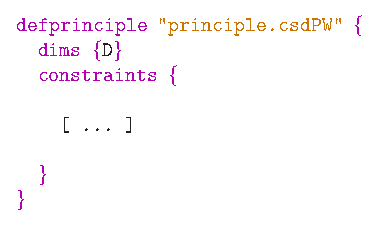
\includegraphics[scale=1.0]{eps/defprinciplecsd}
\end{center}
% \begin{verbatim}
% defprinciple "principle.csdPW" {
%   dims {D}
%   constraints {
    
%     [ ... ]

%   }
% }
% \end{verbatim}

Zu sehen ist, dass in PWUL ein Prinzip analog zur Formalisierung in
XDG aus einem Namen, einer Menge von Dimensionsvariablen und
Constraints besteht. Vor der Prinzipiendefinition ({\tt defprinciple})
selbst k\"onnte man noch Namen an Typen binden mit Ausdr\"ucken wie
{\tt deftype a T}, der den Typ {\tt T} an den Typnamen {\tt a} bindet.
Der Constraint des CSD-Prinzips kann nun als logische Formel
eingef\"ugt werden. Das komplette Prinzip sieht dann so aus:
\begin{center}
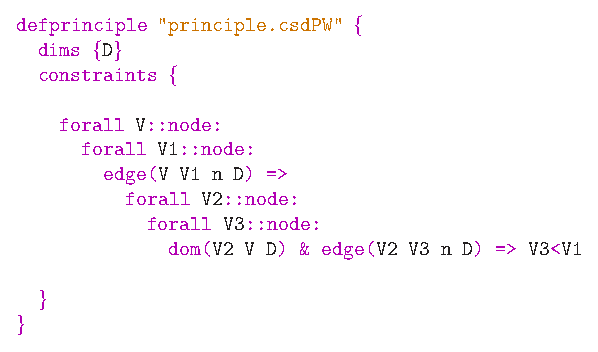
\includegraphics[scale=1.0]{eps/defprinciplecsd1}
\end{center}
% \begin{verbatim}
% defprinciple "principle.csdPW" {
%   dims {D}
%   constraints {
    
%     forall V::node:
%       forall V1::node:
%         edge(V V1 n D) =>
%           forall V2::node:
%             forall V3:node:
%               dom(V2 V D) & edge(V2 V3 n D) => V3<V1

%   }
% }

% \end{verbatim}

Die komplette Liste von Operatoren und Pr\"adikaten der PWUL ist in
Figure~\ref{PWULwords} zu sehen. Die Operatoren der linken Spalte sind
absteigend ihrer Bindungsst\"arke sortiert, wobei die Quantoren gleich
stark binden. Die Operatoren der rechten Spalte binden alle gleich
stark, aber schw\"acher als die Operatoren der linken Spalte.

Figure~\ref{PWULexpr} zeigt die Syntax f\"ur Ausdr\"ucke von Mengen
und Tupel, die auch analog zur XDG Formalisierung gehalten sind. Der
Zugang zu Attributen unterscheidet sich von der XDG Formalisierung, da
man in PWUL auf Attribute zugreifen kann, ohne abfragen zu m\"ussen,
ob ein bestimmtes Tupel in der entsprechenden Menge enthalten ist. In
PWUL liefert der Term {\tt V.D.entry.a} das lexikalische Attribut {\tt
  a} von Knoten {\tt V} in der Dimension {\tt D}. In XDG kann man nur
$(t_1 \ldots t_n) \in a_d(v)$ schreiben. Desweiteren kann man in PWUL
auch Tupel-wertige Attribute haben und nicht nur Mengen von Tupeln wie
in XDG. Typannotationen gibt es in XDG gar nicht, sind f\"ur die
\"Ubersetzung der Formeln in Constraints aber essentiell.

Die erlaubten Typen sind in Figure~\ref{PWULtypes} aufgelistet. Sie
folgen auch der XDG Formalisierung. F\"ur die Typen der rechten Spalte
gilt, dass {\tt Dom} Typen aus der linken Spalte sein m\"ussen.
Desweiteren gilt, dass in der PrincipleWriter User Language alle
Variablen mit einem Gro{\ss}buchstaben beginnen m\"ussen. Konstanten
werden klein geschrieben.

\begin{figure}
\centering
\begin{tabular}{| c | c || c | c |}
\hline
{\bf XDG} & {\bf PWUL} & {\bf XDG} & {\bf PWUL}\\
\hline
$\neg$ & {\tt \verb=~=} & $=$ & {\tt =} \\
$\wedge$ & {\tt \&} & $\neq$ & {\tt \verb=~==} \\
$\vee$ & {\tt $|$} & $\in$ & {\tt in} \\
$\Rightarrow$ & {\tt =>} & $\notin$ & {\tt notin}\\
$\Leftrightarrow$ & {\tt <=>} & $\subseteq$ & {\tt subseteq} \\
$\forall$ & {\tt forall} & $\|$ & {\tt disjoint}\\
$\exists$ & {\tt exists} & $\cap$ & {\tt intersect}\\
$\exists!$ & {\tt existsone} & $\cup$ & {\tt union}\\
 & & $\setminus$ & {\tt minus} \\
\hline
\end{tabular}

\vspace{0.5cm}
\begin{tabular}{| c | c |}
\hline
{\bf XDG} & {\bf PWUL}\\
\hline
$V1 \rightarrow_D V2$  & {\tt edge(V1 V2 D)} \\
$V1 \overset{L}{\rightarrow}_D V2$ & {\tt edge(V1 V2 L D)}\\
$V1 \rightarrow_D^* V2$  & {\tt domeq(V1 V2 D)} \\
$V1 \rightarrow_D^+ V2$  & {\tt dom(V1 V2 D)} \\
$V1 \overset{L}{\rightarrow}_D^+ V2$ & {\tt dom(V1 V2 L D)}\\
$<$ & {\tt <}\\
$w(v) = w $ & {\tt v.word = w}\\
\hline
\end{tabular}
\caption{Operatoren und Pr\"adikate der PWUL}
\label{PWULwords}
\end{figure}

\begin{figure}
\centering
\begin{tabular}{| c | c | c |}
\hline
{\bf XDG} & {\bf PWUL} & \\
\hline
$\{a_1, \ldots ,a_n\}$ & {\tt $\text{\{a}_1 \ldots \text{a}_n \}$} & (Mengen)\\
$(a_1, \ldots , a_n)$ & {\tt $[ \text{a}_1 \ldots \text{a}_n]$ } & (Tupel)\\
$\{(a_1^1 \ldots, a_n^1) \ldots (a_1^k \ldots, a_m^k) \}$ & {\tt
$\text{\{}[\text{a}_1^1 \ldots, \text{a}_n^1] \ldots [\text{a}_1^k
\ldots, \text{a}_m^k] \text{\}}$} & (Mengen von Tupeln)\\
 & {\tt V.D.entry.a} & (Zugang zu
lex. Attributen)\\
 & {\tt V.D.attrs.a} & (Zugang zu nicht-lex. Attributen)\\
 & {\tt V::node} & (Typannotation)\\
\hline
\end{tabular}
\caption{Ausdr\"ucke in PWUL}
\label{PWULexpr}
\end{figure}
\begin{figure}
\centering
\begin{tabular}{| c | c || c | c |}
\hline
{\bf XDG} & {\bf PWUL} & {\bf XDG} & {\bf PWUL}\\
\hline
$\{a_1,\ldots,a_n\}$ & {\tt {\{a$_1$ ... a$_n$\}}} & $2^{Dom}$ & {\tt set(Dom)}\\
$dl ~ D$ & {\tt label(D)} & $Dom_1 \times \ldots \times Dom_n$ & {\tt tuple(Dom$_1
  \ldots$ Dom$_n$)}\\
$V$ & {\tt node} & $2^{Dom_1 \times \ldots \times Dom_n}$ & {\tt set(tuple(Dom$_1
   \ldots $ Dom$_n$))}\\ 
$D$ & {\tt dim} & &\\
$A$ & {\tt attr} & &\\
$W$ & {\tt word} & &\\
\hline
\end{tabular}
\caption{Typen der PWUL}
\label{PWULtypes}
\end{figure}

\subsection{Das Parsermodul des PrincipleWriters}

\begin{figure}
\begin{center}
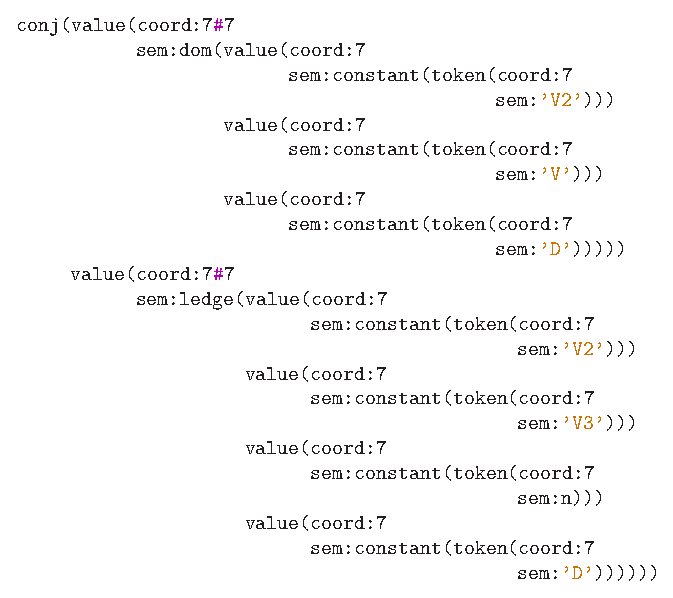
\includegraphics[scale=1.0]{eps/output}
\end{center}
% \begin{verbatim}
% conj(value(coord:7#7 
%            sem:dom(value(coord:7 
%                          sem:constant(token(coord:7 
%                                             sem:'V2'))) 
%                    value(coord:7 
%                          sem:constant(token(coord:7 
%                                             sem:'V'))) 
%                    value(coord:7 
%                          sem:constant(token(coord:7 
%                                             sem:'D'))))) 
%      value(coord:7#7 
%            sem:ledge(value(coord:7 
%                            sem:constant(token(coord:7 
%                                               sem:'V2'))) 
%                      value(coord:7 
%                            sem:constant(token(coord:7 
%                                               sem:'V3'))) 
%                      value(coord:7 
%                            sem:constant(token(coord:7 
%                                               sem:n ))) 
%                      value(coord:7 
%                            sem:constant(token(coord:7 
%                                               sem:'D')))))) 
% \end{verbatim}
\caption{Beispieloutput des Parsers f\"ur: $V2 \rightarrow_D V \wedge
 V2 \overset{n}{\rightarrow}_D V3$}
\label{parseroutput}
\end{figure}

Das Parsermodul des PrincipleWriters besteht aus drei Teilen. Einem
Tokenizer, einer kontextfreien Grammatik und einem Parser.

Sowohl der Tokenizer als auch der Parser stammen aus der
Funktionsbibiliothek von Mozart/Oz. Als Parser kommt ein
LALR-Parser zum Einsatz. Die zugeh\"orige Grammatik wird als
Produktionsregeln in Mozart/Oz Syntax aufgeschrieben. Diese Regeln
k\"onnen in g\"angiger Notation in Anhang~\ref{produktionsregeln}
nachgelesen werden.

Das Parsermodul nimmt ein Prinzip, das in der PrincipleWriter User
Language aufgeschrieben ist als Eingabe. Mit Hilfe des Tokenizers wird
die Eingabe zerlegt. Der Parser baut aus den Tokens und der Grammatik
einen Ableitungsbaum. Der Ableitungsbaum wird als Record realisiert.
Eine vereinfachte Darstellung des Records ist in
Figure~\ref{parseroutput} zu sehen. Im Feld {\tt sem} beginnt ein
neuer Unterbaum, bzw. ein Blatt. Das Feld {\tt coord} bezeichnet die
Zeilennummer des Tokens im Eingabestring, die sp\"ater f\"ur
Fehlermeldungen beim Typchecker verwendet wird.
